\chapter{FEA data management}
\label{chapter:data-management}

% Psat uz rovnou o mem reseni. Zadne okecavani.
% Napsat, ze hodlam vyuzit model Software-as-a-service, popis dat bud do footnote, nebo do kapitoly Concepts.
% Pridat diagram prezentujici cely system - vsechny jeho komponenty (Webapi, Solver, Modeller? - misto toho model importer, Web-based postprocessor, Desktop-based postprocessor, Project Database, Result database)

% project-management, storage-format, modeller (OOFEM-link, script-based engine), post-processors, layer format, filters


\section{System architecture}
\label{sec:system-architecture}

% project management, SQL relational database
% zminit modeller a OOFEM-link, ukazka db modelu
% solution.json
% model attributes: viz clanek FEA with Relational DB, section FEA Data and Dataflow

Figure \ref{fig:FEA-db-schema}, Figure \ref{fig:FEA-db-schema-results}.

\begin{figure}[H]
    \centering
    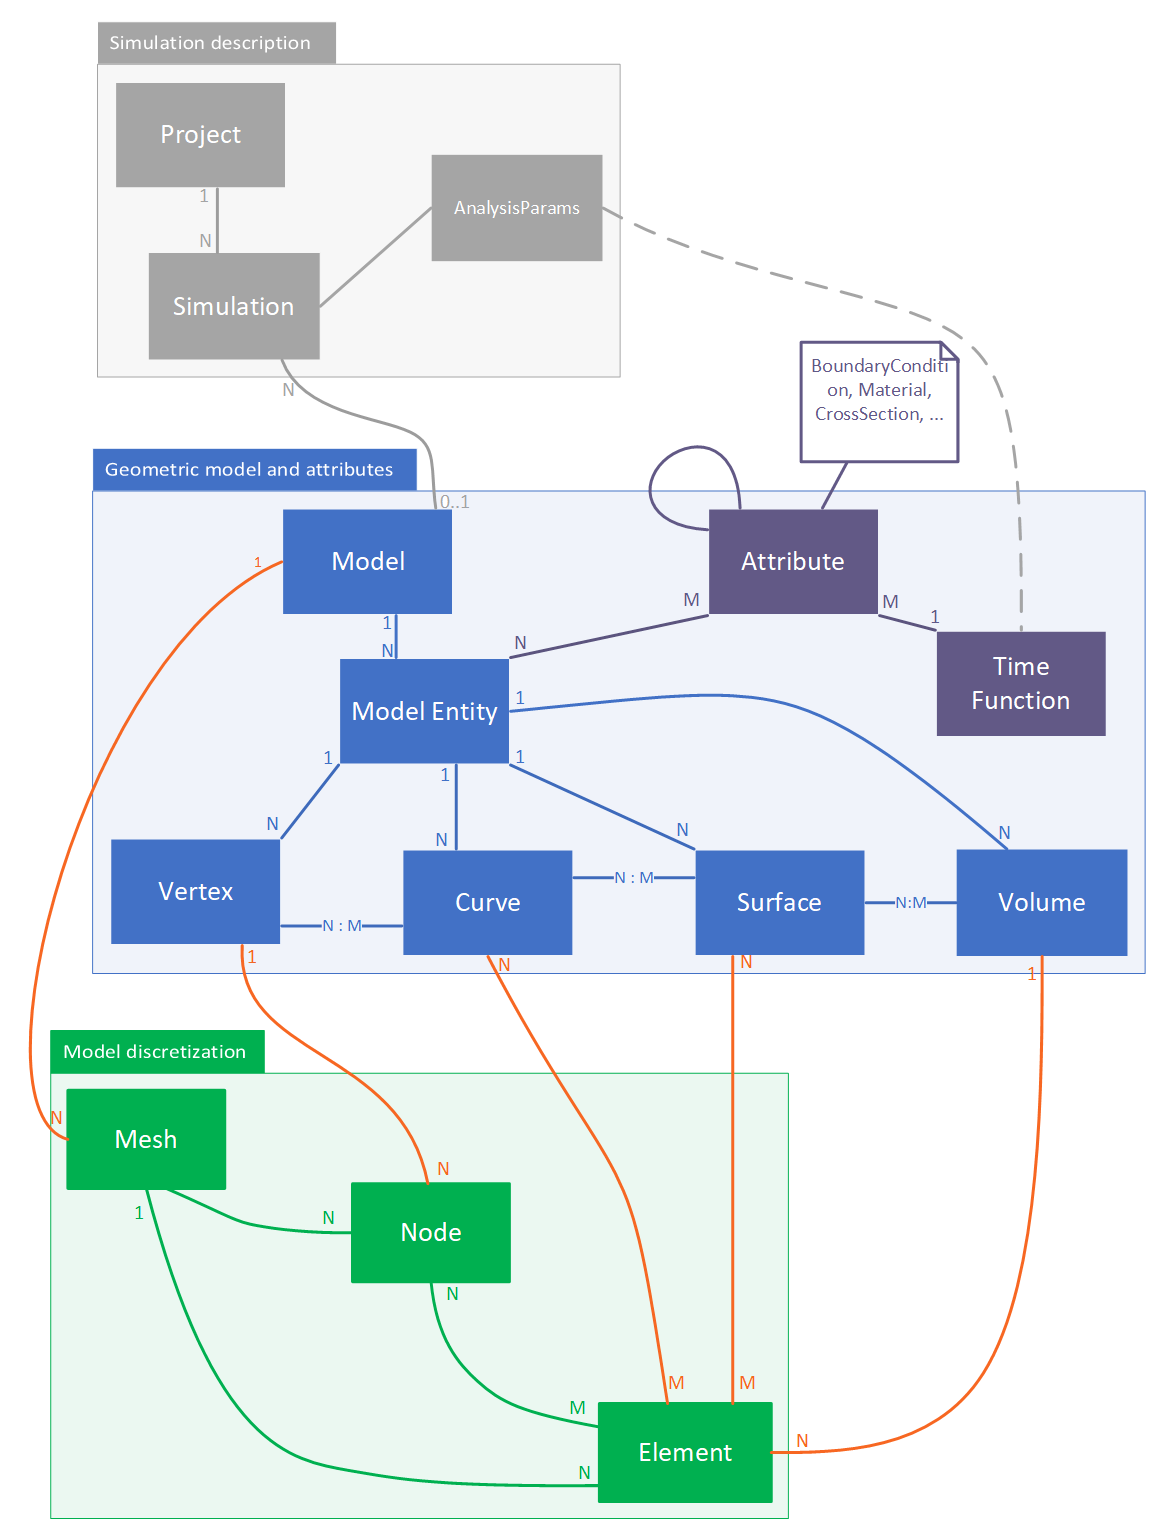
\includegraphics[width=0.8\textwidth]{figures/FEA-database-schema}
    \decoRule
    \caption{Database schema for FEA.}
    \label{fig:FEA-db-schema}
\end{figure}

\begin{figure}[H]
    \centering
    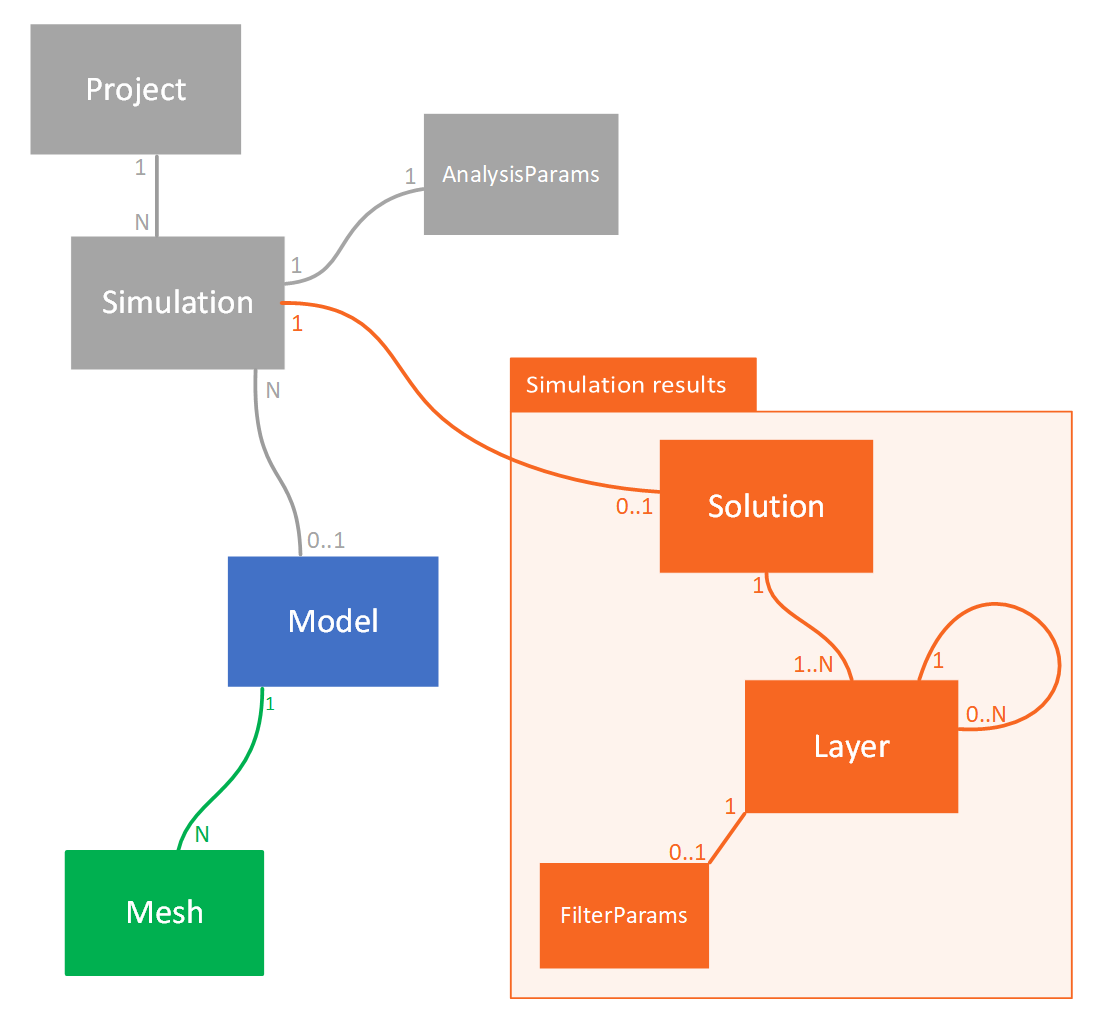
\includegraphics[width=0.7\textwidth]{figures/FEA-database-schema-with-results}
    \decoRule
    \caption{Database schema for FEA with representation of results.}
    \label{fig:FEA-db-schema-results}
\end{figure}

\section{Storage format}
\label{sec:storage-format}

% hodne se inspirovat oznacenymi vetami v clanku FEA-with-relational-DB

% samotny seznam souboru, ktere pouzivam. Nerikat tomu soubory, ale dokumenty? objekty?
% summary.json, mesh.json, attribute.json, and result.json - odkaz do Appendixu na example
% NoSQL DB
% U kazdeho souboru

% konverze z tradicnich souboru do noveho formatu (do budoucna integrovat do solveru); data location Points/Cells/CellPoints, GP extrapolation

\subsection {Encoding}
% base64, JSON, XML, ...

\subsection {Compression}
% Compression methods: SVD, Wavelet, polynomial functions, ... Kazdou rozepsat, u Wavelet zminit Hilbert curve?
% main features for optimization: key time steps (time step span compression), Randomized SVD, Parallelization, Sparse matrix of details, prenasobeni U matice singularnimi cisly, trochu usetrim pamet, mohu pouzit vzorkovani...

\section{Efficient postprocessing}
\label{sec:efficient-postprocessing}

% layers, filters, vytvoreni Surface vrstvy pro webovy postprocessor, barevna skala, Remote/Local solutions - neni rozdil, postprocessor je tenky klient, prepinani skalarnich velicin, vektorove veliciny - je treba nacist vice komponent najednou. Dekomprese: prenasobeni matic - staci jeden radek. ...

\section{Implementation details}
\label{sec:implementation-details}
% implementation details; cloud-infrastructure, Azure functions, web frontend, backend providing project info, blob-storage with layer format; command-based console management; reference to appendix with storage format examples
% SVD compression using redsvd; How is realized postprocessing of compressed data
% Encoding: converting to text representation, base64, NaN values, ... UTF8

% Webový browser, WebGL, textové pole se zadáváním příkazů, veškeré zpracování příkazů na serveru, na klient se budou posílat jen grafické buffery

% Přidat podkapitolku o implementaci barevné škály (diskrétní, spojitá, isoareas shader)

Figure \ref{fig:results-class-diagram}.

\begin{figure}[H]
    \centering
    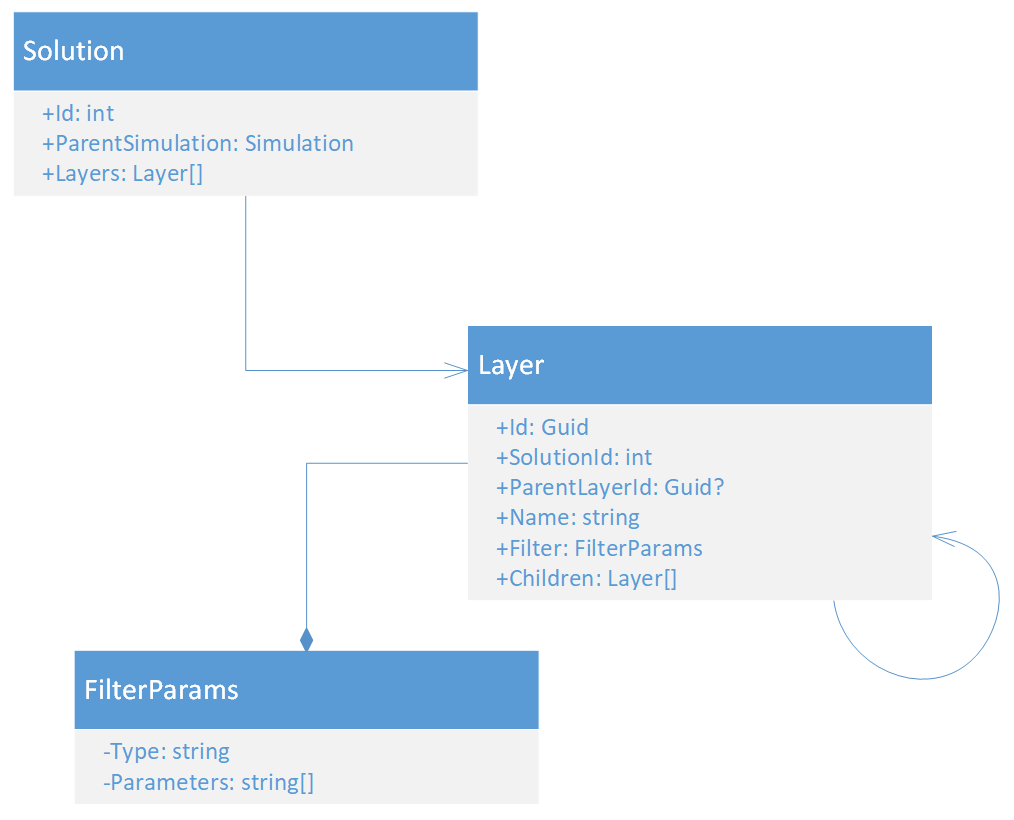
\includegraphics[width=0.7\textwidth]{figures/results-class-diagram}
    \decoRule
    \caption{Class diagram of results representation}
    \label{fig:results-class-diagram}
\end{figure}